\section{Case study}
\label{sec:case study}

\begin{figure}
	\centering
	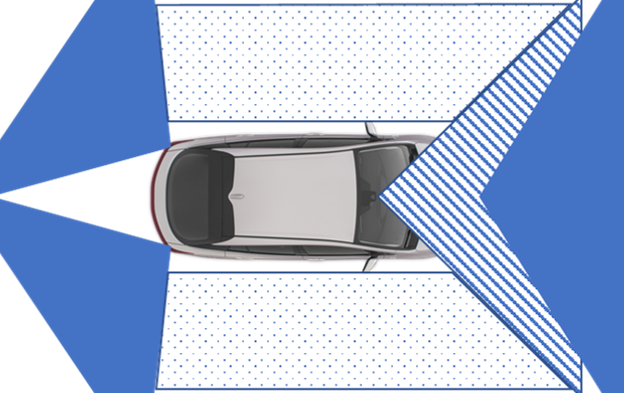
\includegraphics[width=.8\linewidth]{figures/sensors}
	\caption{\cstartd Schematic representation of the field of view of the three radars (solid area) and the camera (area filled with lines) that the ego vehicle is equipped with. The positions of vehicles on the left or the right of the ego vehicle (dotted area) are predicted based on previous measurements.\cendd}
	\label{fig:sensors}
\end{figure}

Here we illustrate the method by applying the method to the dataset described in \autocite{paardekooper2019dataset6000km}.
\cstartd To measure the surrounding traffic, the ego vehicle is equipped with three radars and one camera, as shown in \cref{fig:sensors}.
The images from the camera are used to estimate the lane line distances \autocite{elfring2016effective}.
Furthermore, the surrounding traffic is measured by fusing the data of the radars and the camera \autocite{elfring2016effective}.
While fusing the data of the different sensors, the position of the vehicles that disappear from the sensors' field of view on the left and right of the ego vehicle, see the dotted area in \cref{fig:sensors}, are predicted until the vehicles appear again in the sensors' field of view.
In total, four hours of driving are analyzed.
\cendd

\cstartd To illustrate the proposed scenario mining approach, two different scenario categories are considered: ``cut in'' and ``overtaking before lane change''.
\Cref{fig:cutin formulation tags,fig:overtaking template} show the formulation of these scenario categories using tags.
\Cref{tab:parameters} lists the values of the parameters that are used for the tagging of the data.
\cendd

\begin{figure*}
	\centering
	\setlength{\descriptionwidth}{7em}
\begin{tikzpicture}
% Ego vehicle.
\node[block, text width=\subjectwidth-1em, minimum width=\subjectwidth, fill=egocolor] at (-\descriptionwidth, 0) {Ego vehicle};
\node[block, text width=\descriptionwidth-1em, minimum width=\descriptionwidth, fill=egocolor] at (0, 0) {Lateral activity};
\node[tagitemtwo, fill=egocolor] at (0, 0) {Following lane};
\node[tagitemtwo, fill=egocolor] at (2\itemwidth, 0) {Changing lane left};

% Other vehicle, lateral state.
\node[block, text width=\subjectwidth-1em, minimum width=\subjectwidth, fill=othervehicle, minimum height=2\tagheight] at (-\descriptionwidth, -\tagheight-\tagsep) {Other vehicle};
\node[block, text width=\descriptionwidth-1em, minimum width=\descriptionwidth, fill=othervehicle] at (0, -\tagheight-\tagsep) {Lateral state};
\node[tagitemthree, fill=othervehicle] at (0, -\tagheight-\tagsep) {Left of ego};
\node[tagitem, fill=othervehicle] at (3\itemwidth, -\tagheight-\tagsep) {Same lane as ego};

% Other vehicle, longitudinal state.
\node[block, text width=\descriptionwidth-1em, minimum width=\descriptionwidth, fill=othervehicle] at (0, -2\tagheight-\tagsep) {Longitudinal state};
\node[tagitem, fill=othervehicle] at (0, -2\tagheight-\tagsep) {Behind ego};
\node[tagitemthree, fill=othervehicle] at (\itemwidth, -2\tagheight-\tagsep) {In front of ego};

% Static environment.
\node[block, text width=\subjectwidth-1em, minimum width=\subjectwidth, fill=staticenvironment] at (-\descriptionwidth, -3\tagheight-2\tagsep) {Static environment};
\node[block, text width=\descriptionwidth-1em, minimum width=\descriptionwidth, fill=staticenvironment] at (0, -3\tagheight-2\tagsep) {On highway};
\node[tagitemfour, fill=staticenvironment] at (0, -3\tagheight-2\tagsep) {Highway};

% Items.
\foreach \i in {1, 2, 3, 4} {%
	\node[minimum width=\itemwidth, align=center, minimum height=\itempos, anchor=north east] at (\i\itemwidth, \itempos) {Item \i};
	\draw[showitem] (\i\itemwidth, 0) -- (\i\itemwidth, \itempos);
}
\draw[showitem] (0, 0) -- (0, \itempos);
\end{tikzpicture}
	\caption{\cstartd Formulation of the scenario category ``overtaking before lane change'' using tags.\cendd}
	\label{fig:overtaking template}
\end{figure*}

\begin{table}
	\centering
	\caption{\cstartc Values of parameters used in the case study. \cendc}
	\label{tab:parameters}
	\cstartc
	\begin{tabularx}{\linewidth}{lXl}
		\toprule
		Parameter & Description & Value \\ \otoprule
		$\sampletime$ & Sample time & \SI{0.01}{\second} \\
		$\samplehorizon$ & Sample window & 100 \\
		$\accelerationstart$ & Threshold determining the start of an acceleration or deceleration activity & \SI{0.1}{\meter\per\second\squared} \\
		$\accelerationcruise$ & Threshold determining the end of an acceleration or deceleration activity & \SI{0.1}{\meter\per\second\squared} \\
		$\speeddiff$ & Minimum speed increase/decrease for an acceleration/deceleration activity & \SI{1}{\meter\per\second} \\
		$\samplescruising$ & Minimum number of samples for cruising activity & 400 \\
		$\lanechangethreshold$ & A lane change is detected when the difference between consecutive lane line distances is larger than this threshold & \SI{1}{\meter} \\
		$\lanechangespeed$ & Threshold determining the start and end of a lane change & \SI{0.25}{\meter\per\second} \\
		$\factorgoalmax$ & Maximum factor of the lane width for a lane change of any other vehicle & 0.5 \\
		$\factorgoalmin$ & Minimum factor of the lane width for a lane change of any other vehicle & 0.1 \\
		\bottomrule
	\end{tabularx}
	\cendc
\end{table}

\cstartd The results of the scenario mining are presented in \cref{tab:results}.
A false negative (FN) means that a scenario that occurred is not detected and a false positive (FP) means that the scenario mining detects a scenario whereas this scenario does not occur.
The true positives (TP) are the scenarios that are correctly detected.
The recall is the ratio of the number of true positives (TP) and the total number of scenarios that occur (TP+FN) and the precision is the ratio of the number of true positives (TP) and the total number of detected scenarios (FP+TP).
The F1 score is the harmonic mean of the recall and the precision.
\cendd

\begin{table}
	\centering
	\caption{\cstartd Results of the scenario mining.\cendd}
	\label{tab:results}
	\cstartd
	\begin{tabularx}{\linewidth}{Xr<{\hspace{-1pt}}r<{\hspace{-1pt}}r<{\hspace{-1pt}}r<{\hspace{-1pt}}r<{\hspace{-1pt}}r<{\hspace{-1pt}}}
		\toprule
		Scenario category & FN & FP & TP & Recall & Precision & F1 score \\ \otoprule
		Cut in & 3 & 3 & 33 & \SI{92}{\percent} & \SI{92}{\percent} & \SI{92}{\percent}  \\
		Overtaking before lane change & 1 & 0 & 18 & \SI{95}{\percent} & \SI{100}{\percent} & \SI{97}{\percent} \\
		\bottomrule
	\end{tabularx}
	\cendd
\end{table}

\cstartd As listed in \cref{tab:results}, 33 out of 36 cut ins are correctly detected and 3 out of the 36 detected cut ins are incorrect. 
This results in an F1 score of \SI{92}{\percent}.
For the scenario category ``overtaking before lane change'', 18 out of 19 scenarios are correctly detected and there are no scenarios incorrectly detected.
This results in an F1 score of \SI{97}{\percent}.

The case study illustrates that the performance of the scenario mining is limited by the quality of the data rather than the proposed approach.
The false detections are a result of inaccurate or missing data.
For example, in case of the four false negatives, the other vehicle is not measured at the time of the cut in or overtaking.
For one cut in, this is because another vehicle obstructs the view toward the vehicle at the moment of the cut in. 
For the other three false negatives, the other vehicles appear from the sensor's blind spot (dotted area in \cref{fig:sensors}).
The three false positives of the cut-in scenario are a result of inaccurate measurements of the lane line distances.
\cendd
